%\documentclass[xcolor=dvipsnames,compress,handout]{beamer}
\documentclass[xcolor=dvipsnames,compress]{beamer}
\usepackage[utf8]{inputenc}
\usepackage[english]{babel}
\usepackage{pgf}
\usepackage{graphicx}
\graphicspath{ {images/} }
\usepackage[absolute,overlay]{textpos}
\usepackage{xcolor}
\usepackage{comment}
\usepackage{xpatch}
\usepackage{tabularx}
\usepackage[export]{adjustbox}
\usepackage{pgffor}
\usepackage{blindtext}
\usepackage{multirow}
\usepackage{algpseudocode} % Pseudocode
\usepackage{algorithm} % Float for algorithms

% DESIGN
\definecolor{RUBblue}{rgb}{0,0.21,0.38}
\definecolor{AIblue}{rgb}{0,0.57,0.87}

% DO NOT ASK WHAT HAPPENS HERE
% Okay...
\useoutertheme[subsection=false]{miniframes}
\usecolortheme{beaver}
\beamertemplatenavigationsymbolsempty
\setbeamertemplate{footline}{%
	\begin{beamercolorbox}[wd=\paperwidth,ht=0ex,left]{default}
		%\insertauthor\hfill\insertframenumber%
		\colorbox{AIblue}{\vphantom{2cm}\hspace{14cm}}
	\end{beamercolorbox}
}
\setbeamercolor{item}{fg=RUBblue}
\setbeamercolor{title}{fg=Black}
\setbeamercolor{frametitle}{fg=Black}
\setbeamerfont{title}{size=\large}
\setbeamertemplate{itemize items}[square]
\setbeamercolor{section in head/foot}{bg=AIblue}
\setbeamerfont{footline}{size=\fontsize{15}{12}\selectfont}


\xpatchcmd{\itemize}
	{\def\makelabel}
	{\setlength{\itemsep}{0.2cm}\def\makelabel}{}{}

 
\addtobeamertemplate{frametitle}{}{
\begin{textblock*}{100mm}(1.01\textwidth,0.65cm)
	
\includegraphics[height=0.7cm]{logo-ai.png}
\end{textblock*}}

% COMMANDS
\DeclareMathOperator{\sign}{sign}
\renewcommand{\vec}[1]{\underline{#1}}
\newcommand{\mat}[1]{\underline{\underline{#1}}}
\newcommand{\abs}[1]{\left\lvert#1\right\rvert}
\newcommand\braces[1]{\left(#1\right)}
\newcommand\brackets[1]{\left[#1\right]}
\newcommand\NEWLINECOMMENT[1]{\STATE\STATE/* #1 */}
\newcommand\Only[2]{\only<#1|handout:#1>{#2}}
\newcommand\overlayImage[6]{
	\only<#1|handout:#2>{
		\begin{textblock*}{\textwidth}(#3cm,#4cm)
			\frame{
				\includegraphics[width=#5\textwidth]{#6}
			}
		\end{textblock*}
	}
}





% TITLEPAGE
\title{\textbf{Exploring Ways to Harden Deep Convolutional Neural Networks against Constructed Adversarial Examples}}
\author{Christian Andreas Mielers}
\institute{Ruhr-University Bochum\\Institute for Neural Computation\\Master thesis presentation}
\date{19th of December 2016}
 
\begin{document}
%\section{Titlepage}
%\subsection{Titlepage}
\maketitle





\section{Introduction}
\subsection{Introduction}

\frame{
	\frametitle{Adversarial Examples}
	\begin{columns}
		\column{0.5\textwidth}
			\begin{itemize}
				\item<1-> GoogLeNet
				\only<1>{
					\item Prediction \emph{giant panda}, $99.23\%$ confidence
				}
				\only<2->{
					\item Prediction \emph{acorn}, $86.17\%$ confidence
				}
				\item<3-> Elicits erroneous prediction with minimal changes
			\end{itemize}
		\column{0.4\textwidth}
			\only<1>{
				\begin{figure}
					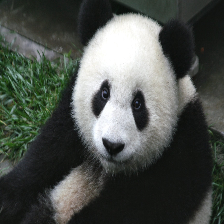
\includegraphics[width=\textwidth]{aes/panda}
					\caption{Original image}
				\end{figure}
			}
			\only<2->{
				\begin{figure}
					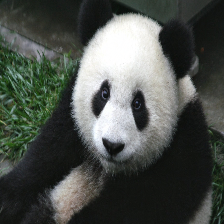
\includegraphics[width=\textwidth]{aes/panda_acorn_10_0dot9}
					\caption{Adversarial example}
				\end{figure}
			}
	\end{columns}
}

%\frame{
%	\frametitle{Neural Networks}
%	\begin{columns}
%		\column{0.5\textwidth}
%			\begin{itemize}
%				\item Drastic simplification from biology
%				\item First operation is a dot product
%				\item Activation function breaks linearity
%				\item<2-> Organized in layers
%				\item<2-> Every neuron is connected to all neurons in adjacent layers
%			\end{itemize}
%		\column{0.5\textwidth}
%			\includegraphics<1>[width=\textwidth]{artificial_neuron} % TODO remove indices
%			\includegraphics<2>[width=\textwidth]{network_layout} % TODO remove indices
%	\end{columns}
%}

%\frame{
%	\frametitle{Convolutional Neural Networks}
%	\begin{columns}
%		\column{0.5\textwidth}
%			\begin{itemize}
%				\item Neuron only connects to local patch
%				\item Weight sharing
%				\item Drastic reduction in number of parameters
%				\item Focus on local features
%				\item<2-> Allows for many filters
%				\item<2-> Organized in maps
%				\item<3-> Reduces map size
%				\item<3-> Improves translation invariance
%			\end{itemize}
%		\column{0.5\textwidth}
%			\includegraphics<1>[width=\textwidth]{convolution_layer}
%			\includegraphics<2>[width=\textwidth]{convolution_layer_maps}
%			\includegraphics<3>[width=\textwidth]{pooling_layer}
%	\end{columns}
%}





\section{Adversarial Examples}
\subsection{Adversarial Examples}

\frame{
	\frametitle{Fast Gradient Sign Method}
	\begin{itemize}
		\item Backpropagate to optimize the \emph{image \vec{i}}
		\item Use the gradient of the loss function $J$ w.r.t \vec{i}
		\item Provide false label $l$
		\item Modulate strength via $c$
	\end{itemize}
	
	\begin{align*}
		\vec{r} &= c \cdot \sign \braces{\nabla_\vec{i} J \braces{\vec{\theta}, \vec{i}, l}}
	\end{align*}
}

\frame{
	\frametitle{Iterative Fast Gradient Sign Method}
	\newcommand\numIt{\text{num\_iterations}}
	\newcommand\advEx{\text{ae}}
	\newcommand\grad{\text{grad}}
	\footnotesize{
		\begin{algorithmic}
			\Function{IterativeFGSM}{input\_data, l, c, \numIt}
				\State \advEx $\ \gets$ input\_data
				\State $i \gets 0$
				\While{$i < \numIt$}
					\State $\grad \gets$ \Call{Network.Backprop}{\advEx, l}
					\State $r \gets \frac{c}{\numIt} \cdot \sign \braces{\grad[0]}$ \Comment{grad[0] indicates input gradient}
					\State \advEx $\ \gets$ $\advEx + r$
					\State $i \gets i + 1$
				\EndWhile
				\State \Return \advEx
			\EndFunction
		\end{algorithmic}
	}
}

\frame{
	\frametitle{Differences and Gradients}
	\begin{columns}
		\column{0.4\textwidth}
			\begin{figure}
					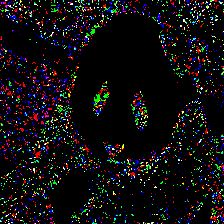
\includegraphics[width=\textwidth]{aes/panda_acorn_10_0dot9_posdiff}
					\caption{Positive pointwise difference, $98\%$ percentile}
				\end{figure}
		\column{0.4\textwidth}
			\begin{figure}
				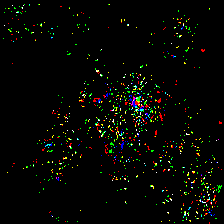
\includegraphics[width=\textwidth]{aes/panda_acorn_10_0dot9_grad}
				\caption{Gradient sign, scaled by $98\%$ percentile}
			\end{figure}
	\end{columns}
}
%TODO note differences

\frame{
	\frametitle{Confidence}
	\begin{columns}
		\column{0.5\textwidth}
			\begin{itemize}
				\item Increasing iteration count improves confidence
				\item Quickly levels off
				%\item Acorn reaches $\approx 95\%$, Dresser only $\approx 2\%$
				\item<2-> Higher $c$ allows more transformations to succeed
				\item<2-> Dresser curve is delayed and slower
				\item<3-> Striking visual artifacts
			\end{itemize}
		\column{0.5\textwidth}
			\only<1>{
				\begin{figure}
					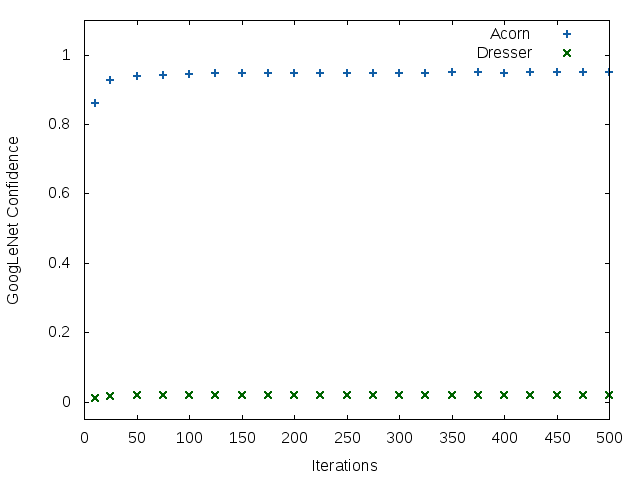
\includegraphics[width=\textwidth]{confidence-vs-iterations}
					\caption{Confidence w.r.t. iteration count, $c = 0.9$}
				\end{figure}
			}
			\only<2>{
				\begin{figure}
					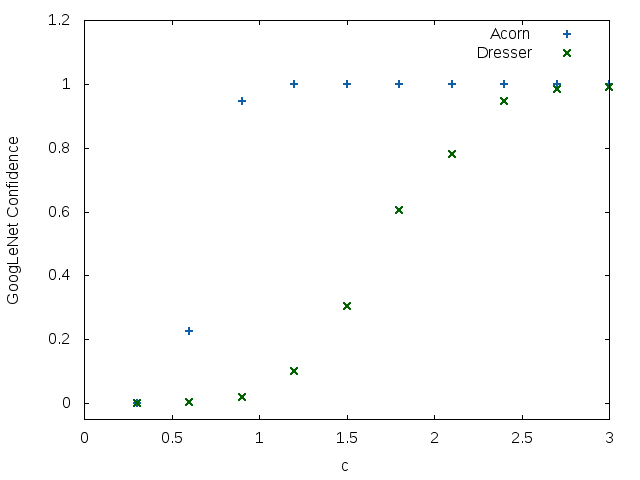
\includegraphics[width=\textwidth]{confidence-vs-coeff}
					\caption{Confidence w.r.t. adaption strength coefficient, 100 iterations each}
				\end{figure}
			}
			\only<3>{
				\begin{figure}
					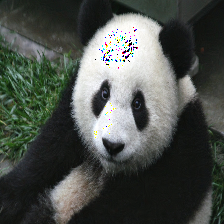
\includegraphics[width=0.8\textwidth]{aes/panda_dresser_100_1dot8}
					\caption{100 iterations, $c=1.8$}
				\end{figure}
			}
	\end{columns}
}

\frame{
	\frametitle{Iterative confidence development}
	\begin{columns}
		\column{0.5\textwidth}
			\begin{itemize}
				\item Source class probability declines before adversarial probability rises
				\item Minimal combined probability after iteration 53
				\item<2-> Probability is distributed to unrelated classes
				\item<3-> Sigmoidal shape
			\end{itemize}
		\column{0.5\textwidth}
			\only<1,3>{
				\begin{figure}
					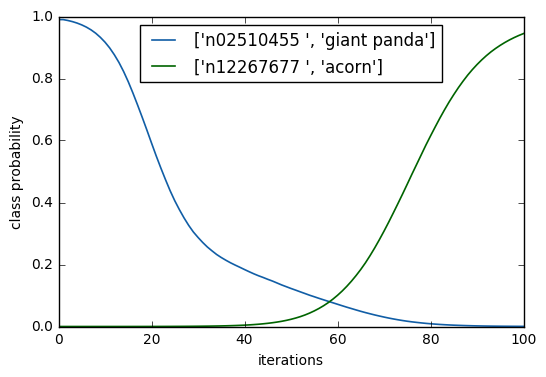
\includegraphics[width=\textwidth]{confidence-evolution-100}
					\caption{Confidence w.r.t. iteration, $c = 0.9$}
				\end{figure}
			}
			\only<2>{
				\begin{tabular}{|l|l|}
					\hline
					Class & Probability \\
					\hline
					giant panda & 0.1064 \\
					teddy & 0.0929 \\
					hamster & 0.0433 \\
					acorn & 0.0371 \\
					custard apple & 0.0364 \\
					\hline
				\end{tabular}
			}
	\end{columns}
}





\section{AE Batches}
\subsection{AE Batches}

\frame{
	\frametitle{GTSRB}
	\begin{figure}
		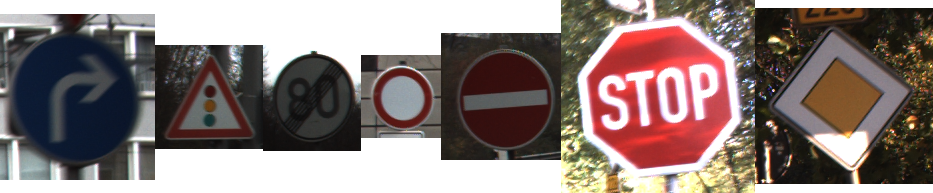
\includegraphics[width=\textwidth]{gtsrb/overview}
		%\caption{}
	\end{figure}
	
	\begin{itemize}
		\item German traffic signs organized into 43 classes
		\item Unbalanced class probabilities
		\item $39.209$ training and $12.630$ test images
	\end{itemize}
}

\frame{
	\frametitle{GTSRB Challenges}
	\begin{columns}
		\column{0.5\textwidth}
			\begin{itemize}
				\item Blur
				\item<2-> Overexposure
				\item<3-> Similarity
				\item<4-> Low resolution
				\item<5-> Low contrast
				\begin{itemize}
					\item<6-> Contrast normalization
				\end{itemize}
			\end{itemize}
		\column{0.4\textwidth}
			\includegraphics<1>[width=0.75\textwidth]{gtsrb/problems/class23_00003_00029}
			\includegraphics<2>[width=0.75\textwidth]{gtsrb/problems/class26_00014_00029}
			\includegraphics<3>{gtsrb/problems/class09_00004_00029}
			
			\includegraphics<3>{gtsrb/problems/class10_00025_00029}
			\includegraphics<4>{gtsrb/problems/class28_00012_00003}
			\includegraphics<5>[width=0.75\textwidth]{gtsrb/problems/class19_00004_00029}
			\includegraphics<6>[width=0.75\textwidth]{gtsrb/problems/class19_00004_00029_normalized_contrast}
	\end{columns}
}

\frame{
	\frametitle{GTSRB Network}
	\centering
	\footnotesize{
		\begin{tabular}{llll}
			\textbf{Layer} & \textbf{Type} & \textbf{Configuration} & \textbf{Activation function} \vspace{0.25cm} \\
			\hline \\
			0 & Input & $3 \times 48 \times 48$ & - \\
			1 & Convolution & 300 kernels of size $7 \times 7$, & tanh \\
			& & producing 100 maps & \\
			2 & Max-Pooling & Area $2\times 2$, stride 2 & - \\
			3 & Convolution & 15000 kernels of size $4 \times 4$, & tanh \\
			& & producing 150 maps & \\
			4 & Max-Pooling & Area $2\times 2$, stride 2 & - \\
			5 & Convolution & 37000 kernels of size $4 \times 4$, & tanh \\
			& & producing 250 maps & \\
			6 & Max-Pooling & $2\times 2$, stride 2 & - \\
			7 & Fully connected & 300 neurons, with bias term & tanh \\
			8 & Fully connected & 43 neurons, with bias term & softmax \\
		\end{tabular}
	}
}

\frame{
	\frametitle{GTSRB AE Batches}
	\begin{columns}
		\column{0.5\textwidth}
			\begin{itemize}
				\item Cross-generation of AEs
				\item All pairs of source and target class
				\item 500 iterations
				\item 1849 AEs per batch
			\end{itemize}
		\column{0.5\textwidth}
			\centering
				\begin{tabular}{ll}
					\textbf{Batch name} & \textbf{c} \vspace{0.25cm} \\
					\hline \\
					gtsrb-ae-0.005 & 0.005 \\
					gtsrb-ae-0.025 & 0.025 \\
					gtsrb-ae-0.037 & 0.037 \\
					gtsrb-ae-0.05 & 0.05 \\
					gtsrb-ae-0.1 & 0.1 \\
					gtsrb-ae-0.5 & 0.5 \\
					gtsrb-ae-0.9 & 0.9 \\
				\end{tabular}
	\end{columns}
}

\frame{
	\frametitle{ImageNet}
	% images within one class are very diverse
	\begin{columns}
		\column{0.5\textwidth}
			\begin{itemize}
				\item ILSVRC2012 subset
				\item<2-> 1000 classes with a much broader scope
				\item<8-> $1.281.167$ images
				\item<9-> High image quality
				\item<10-> Strong variation within one class
			\end{itemize}
		\column{0.4\textwidth}
			\includegraphics<2>[width=\textwidth]{imagenet/examples/n01820546_31}
			\includegraphics<3>[width=\textwidth]{imagenet/examples/n03530642_10006}
			\includegraphics<4>[width=\textwidth]{imagenet/examples/n02281406_10006}
			\includegraphics<5>[width=\textwidth]{imagenet/examples/n04597913_10021}
			\includegraphics<6>[width=0.75\textwidth]{imagenet/examples/n03937543_10012}
			\includegraphics<7-10>[width=0.75\textwidth]{imagenet/examples/n02782093_1001}
			\includegraphics<11->[width=0.75\textwidth]{imagenet/examples/n02782093_40}
	\end{columns}
}

\frame{
	\frametitle{ImageNet AE Batches}
	\begin{itemize}
		\item Using GoogLeNet for gradients
		\item 500 iterations
	\end{itemize}
	
	\vspace{1cm}
	
	\centering
	\footnotesize{
		\begin{tabular}{llrrr}
			\textbf{Batch name} & \textbf{c} & \textbf{source cl.} & \textbf{target cl.} & \textbf{number of AEs} \vspace{0.25cm} \\
			\hline \\
			imagenet-ae-50 & 0.9 & 50 & 50 & 2500 \\
			imagenet-ae-1000 & 0.9 & 1 & 1000 & 1000 \\
			imagenet-ae-10-3.0 & 3.0 & 10 & 10 & 100 \\
		\end{tabular}
	}
}





\section{Spectra}
\subsection{Spectra}

\frame{
	\frametitle{imagenet-ae-50 spectra}
	\begin{itemize}
		\item Log spectra computed on original data and imagenet-ae-50
		\item Only AEs with confidences $> 0.5$
		\item Difference shows wedge-like pattern
	\end{itemize}
	
	\vspace{0.5cm}
	
	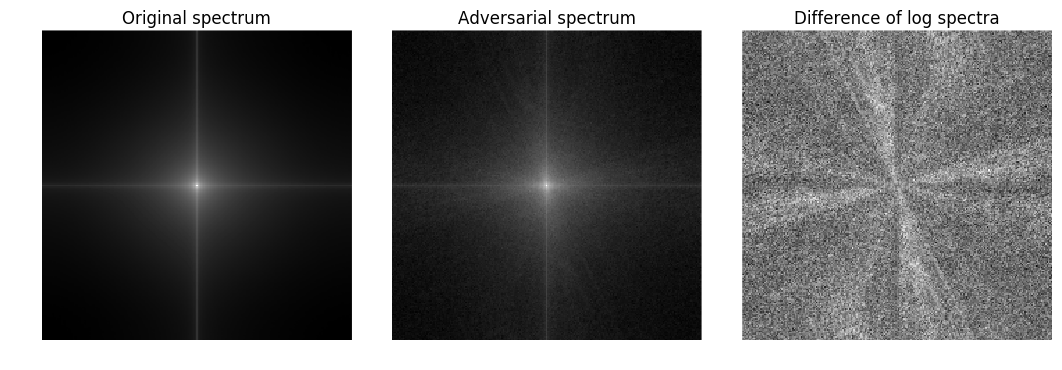
\includegraphics[width=\textwidth]{spectra/imagenet-ae-50-minconfidence-0dot5-maxorig-20000-spectra}
}

\frame{
	\frametitle{imagenet-ae-50 frequency distribution}
	\begin{itemize}
		\item 158 bins
		\item Both distributions are approximately log-linear
		\item Difference reveals mostly higher amplitudes, except for high frequencies
	\end{itemize}
	
	\vspace{0.5cm}
	
	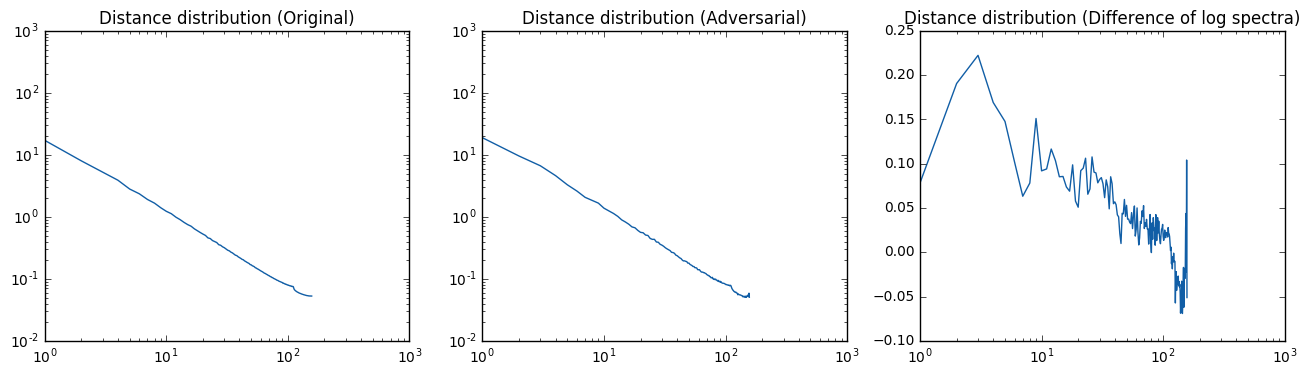
\includegraphics[width=\textwidth]{spectra/imagenet-ae-50-minconfidence-0dot5-maxorig-20000-distance-158-bins}
}

\frame{
	\frametitle{imagenet-ae-50 angle distribution}
	\begin{itemize}
		\item 16 bins
		\item Observable differences w.r.t orientation
	\end{itemize}
	
	\vspace{0.5cm}
	
	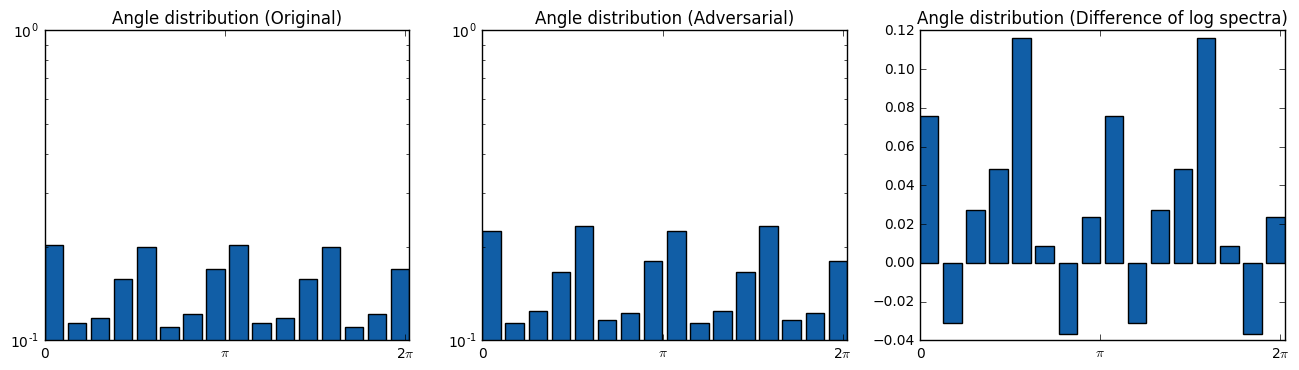
\includegraphics[width=\textwidth]{spectra/imagenet-ae-50-minconfidence-0dot5-maxorig-20000-angle-16-bins}
}

\frame{
	\frametitle{gtsrb-ae-0.025 spectra}
	\begin{itemize}
		\item Log spectra computed on original data and gtsrb-ae-0.025
		\item Only AEs with confidences $> 0.5$
	\end{itemize}
	
	\vspace{0.5cm}
	
	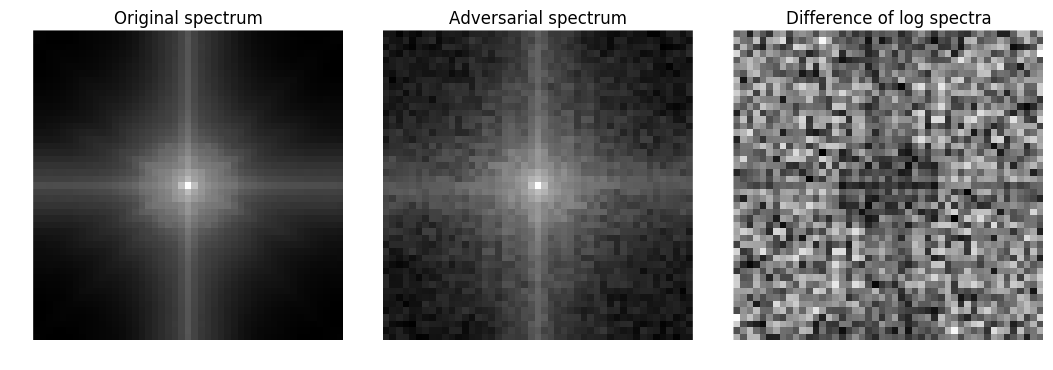
\includegraphics[width=\textwidth]{spectra/gtsrb-ae-0dot025-minconfidence-0dot5-maxorig-0-spectra}
}

\frame{
	\frametitle{gtsrb-ae-0.025 frequency distribution}
	\begin{itemize}
		\item 33 bins
		\item Both distributions are approximately log-linear
		\item Difference reveals mostly higher amplitudes, \emph{especially} for high frequencies
	\end{itemize}
	
	\vspace{0.5cm}
	
	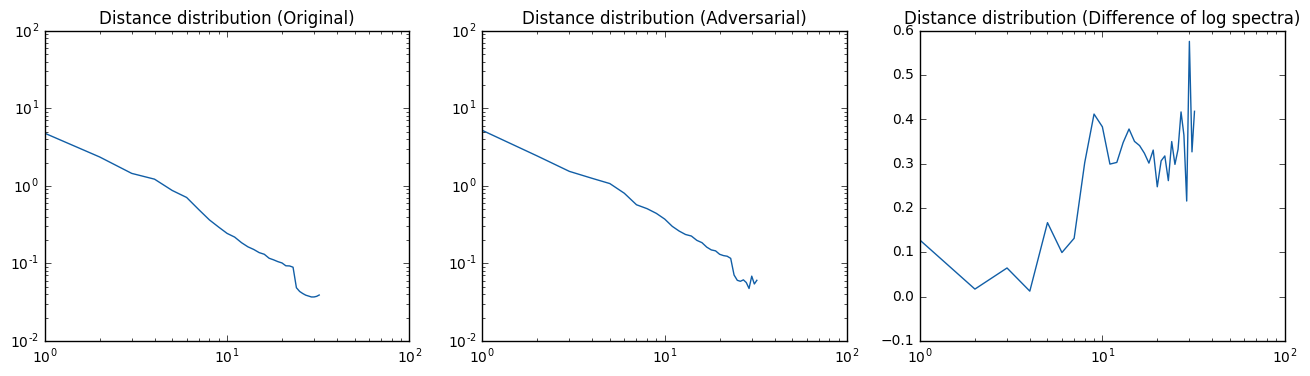
\includegraphics[width=\textwidth]{spectra/gtsrb-ae-0dot025-minconfidence-0dot5-maxorig-0-distance-33-bins}
}

\frame{
	\frametitle{gtsrb-ae-0.025 angle distribution}
	\begin{itemize}
		\item 16 bins
		\item Observable differences w.r.t orientation
	\end{itemize}
	
	\vspace{0.5cm}
	
	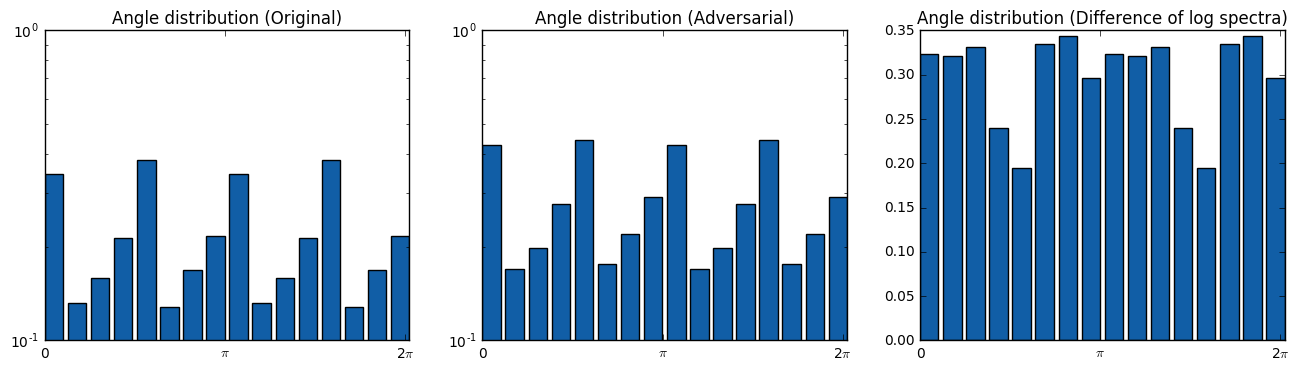
\includegraphics[width=\textwidth]{spectra/gtsrb-ae-0dot025-minconfidence-0dot5-maxorig-0-angle-16-bins}
}





\section{Conversion Compatibility}
\subsection{Conversion Compatibility}

\frame{
	\frametitle{Cross-class conversion in imagenet-ae-50}
	\begin{itemize}
		\item Inspect how well some classes are turned into others
		\item imagenet-ae-50
		\item Confusion-matrix-like plot
	\end{itemize}
}

\frame{
	\centering{
		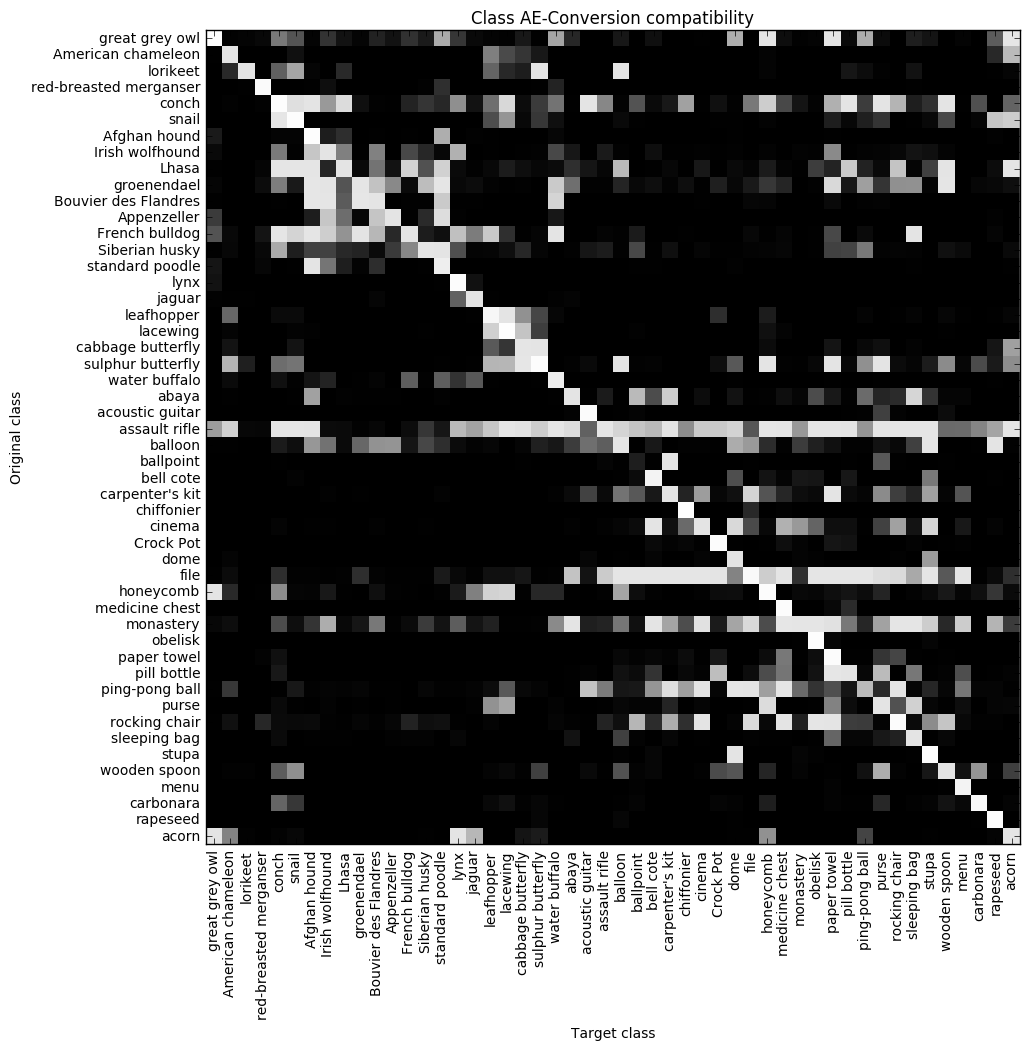
\includegraphics[width=0.75\textwidth]{confusion-matrices/imagenet-ae-50}
	}
}

\frame{
	\frametitle{Cross-class conversion in gtsrb-ae}
	\begin{itemize}
		\item Only one source image per class in imagenet-ae-50
		\item Effects could be influenced by specific image rather than class
		\item Take average confidence of
			\begin{itemize}
				\item gtsrb-ae-0.005
				\item gtsrb-ae-0.025
				\item gtsrb-ae-0.037
				\item gtsrb-ae-0.05
			\end{itemize}
	\end{itemize}
}

\frame{
	\frametitle{gtsrb-ae confusion matrix}
	\centering{
		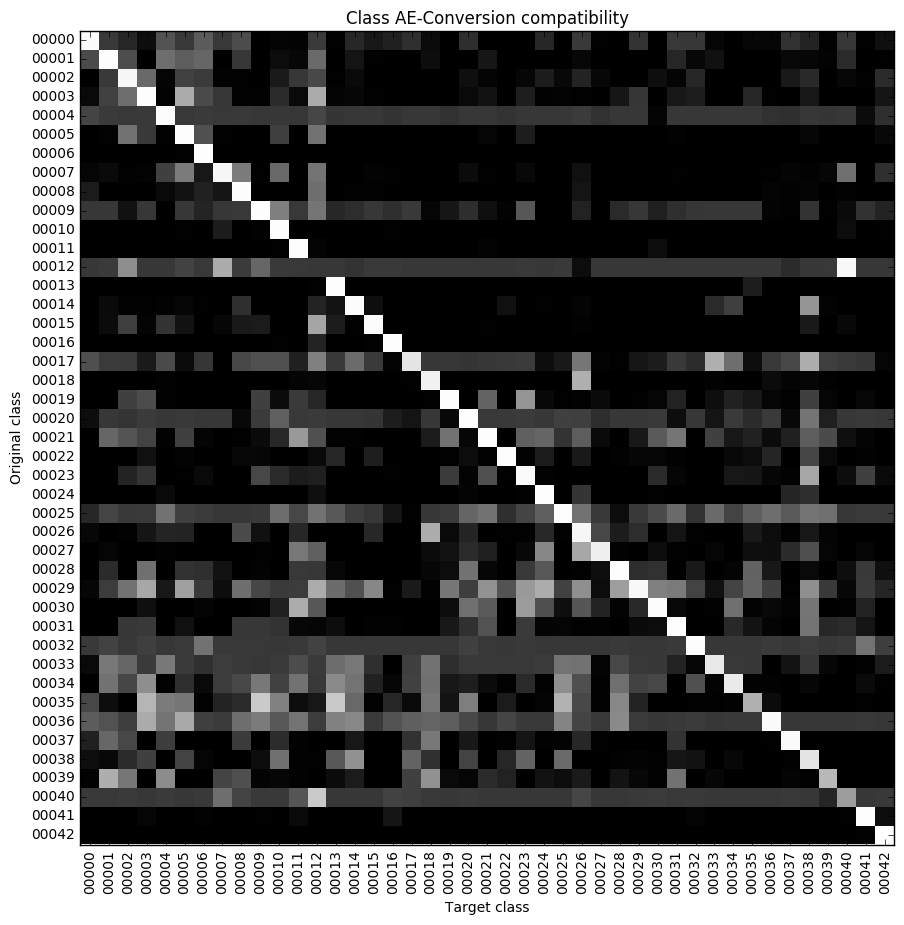
\includegraphics[width=0.65\textwidth]{confusion-matrices/gtsrb-ae-multiple-0005-0025-0037-005}
	}
}

\section{Predicting Confidence}
\subsection{Predicting Confidence}

\frame{
	\frametitle{Fitting sigmoidal functions}
	\begin{itemize}
		\item Confidence evolution looks sigmoidal
		\item Fit parameterized sigmoid
		\item Predict final confidence early on
		\item Problematic because fit mostly happens on constant part
	\end{itemize}
	\only<2>{
		\begin{align*}
			\sigma \braces{x, \alpha, \beta, x_0} &= \frac{\beta}{1 + e^{-\alpha \braces{x - x_0}}}
		\end{align*}
	}
}

\frame{
	\frametitle{Fit results}
	\begin{columns}
		\column{0.5\textwidth}
			\begin{itemize}
				\item 800 curves from ImageNet, with 100 iterations and $c = 0.9$
				\item Initialize with $\alpha = 0.002$, $\beta = 0.5$, $x_0 = 70$
				\item Constraints: $\alpha \geq 0$, $\beta \in \brackets{0, 1}$
				\item Fit on first $40\%$ of iterations
			\end{itemize}
		\column{0.5\textwidth}
			\includegraphics<2>[width=\textwidth]{progress/imagenet_0dot9c_100iter_800samples-success}
			\includegraphics<3>[width=\textwidth]{progress/imagenet_0dot9c_100iter_800samples-failure}
	\end{columns}
}

\frame{
	\frametitle{Predictive power}
	\begin{columns}
		\column{0.5\textwidth}
			\begin{itemize}
				\item Predict whether confidence will be $\geq 0.5$
				\item<2-> Precision $0.5741$
				\item<2-> Recall $0.3563$
				\item<2-> Losing about $65\%$ of AEs
			\end{itemize}
		\column{0.5\textwidth}
			\only<2->{
				\begin{tabular}{ll|ll}
					& & \multicolumn{2}{c}{Prediction} \\
					& & $\geq 0.5$ & $< 0.5$ \\
					\hline
					\multirow{2}{*}{Data} & $\geq 0.5$ & 31 & 56 \\
					& $< 0.5$ & 23 & 690 \\
				\end{tabular}
			}
	\end{columns}
}





\section{Conclusion}
\subsection{Conclusion}

\frame{
	\frametitle{Conclusion}
	\begin{itemize}
		\item Iteratively generating AEs improves quality
		\item Some source-target class pairs require salient changes
		\item During the process probability distributes to other classes
		\item Changes in spectra are data set or network specific
		\item Some classes are great sources for AEs
		\item Some classes are good targets
		\item Similar classes can work well
		\item Predicting final confidence by curve fitting doesn't work well
	\end{itemize}
}

\frame{
	\frametitle{Questions?}
	\begin{figure}[h!]
			\frame{
				
\includegraphics[width=7cm]{fragen.png}
			}
	\end{figure}
}























%\section{Reservoir}
%\subsection{Reservoir}

%\frame{
%	\frametitle{Convolutional Neural Networks}
%	\begin{textblock*}{1.1\textwidth}(0.5cm,2.9cm)
%		\footnotesize{
%			\begin{tabularx}{\textwidth}{cp{0.16\linewidth}p{0.4\linewidth}X}
%			\textbf{Layer} & \textbf{Type} & \textbf{Configuration} & \textbf{Activation function} \\
%			& & & \\
%			\hline
%			& & & \\
%			0 & Convolutional & 100 filters of size $7\times7$ per channel & $\tanh$ \\
%			\end{tabularx}
%		}
%	\end{textblock*}
%	\Only{2}{
%		\begin{textblock*}{1.1\textwidth}(0.95cm,4.0cm)
%			\frame{
%				\includegraphics[width=0.92\textwidth]{images_old/convolutional_networks/tanh}
%			}
%		\end{textblock*}
%	}
%	\Only{3}{}
%}

\end{document}

% TODO Subsections